\chapter{Design}
\label{ch:design}

This chapter introduces the architecture we developed based on the discussion of the requirements and challenges from Chapter~\ref{ch:rqrmsandclngs}. We discuss in detail the implementation of the core components that make the backend of our solution, as the most critical challenge we aim to tackle is to achieve the required performances to make our software usable. We will also discuss the frontend's design, in order to complete our discussion of the architecture, but its implementation and related challenges are out of the scope of this thesis.

%This chapter introduces the design choices implemented in our solution in order to overcome the challenges presented in Chapter~\ref{ch:unmaintainability}. We also discuss the implementation of the most critical aspects of this solution. We do not discuss the \acrshort{ui} implementation as it is out of the scope of this thesis. However, we will still discuss its design as it is part of the architecture we present and tackles some important points that are part of the requirements for the environment we are developing.

%This chapter presents the challenges encountered creating the system, what the most critical components are and the choices we made to overcome said issues. We first present the components that build up the system, what their responsibility are and the choices that lead us to this design. Then tackle each component one by one, focusing separately on each challenge. Afterwards we combine all the choices and present the final architecture of the system developed.

\section{Components}
\label{sec:components}

Based on our discussion of the challenges in Chapter~\ref{ch:rqrmsandclngs}, we opt for an architecture with components that each have a precise separate concern \cite{Hursch95separationof}. This stems from maintainability driven considerations arising from previous work's code, where components were highly coupled with both the visualization library and the engine \cite{dreuning_visual_2016, duking_potential_2018, kruis_creating_2017}. On the other hand, VtkToUnity already implements its code separating the Unity interface from the VTK and visualization logic within the plugin, moving most of its complexity in the C\# scripts.

The most basic design of our architecture requires two main endpoints, that are \acrshort{vtk} and Unity, a native layer of interfacing between the two and a managed Unity plugin to manage the invocation of native code from managed level and to implement the VR app's logic. The bare bones implementation was developed by Wheeler et al. \cite{wheeler_virtual_2018}, on which our solution is based. This gives us an infrastructural basement on which our further components are then built.

To achieve our goal of full integration of VTK, we cannot rely on hardcoded functions, which would impair the generality of the system, as well as its maintainability. As such, our solution comprises an introspecting component that enables the gathering of metadata on \acrshort{vtk} and thus limits the coupling of the solution to a particular version of \acrshort{vtk}.

On the other hand, the expression of such metadata also needs to be lowly coupled with the particular implementation of \acrshort{vtk}, and as such a component is introduced to enable the generation on-the-fly of UI that fits the I/O operations required to support the development environment. The design of the UI parts themselves is out of the scope of this thesis; we will only discuss its design, which enables the creation of the UIs.

Finally, this generality may come at the price of performance as introspection may be slow and interfacing may not be complete through it, as we discuss in Section~\ref{sec:design-introspection}, and the UI generation may be slow when working with big and complex pipeline filters. A first experiment in Section~\ref{sec:rqrmsandclngs-validation} shows that the performance on the creation of a somewhat complex pipeline using introspection, which yielded promising results. However, these performances may not be enough in all cases to support the use we envision for this software. As such, to enable users to enhance their experiences, both  tailored, more user-friendly UIs as well as focused and efficient adapters that create a direct link between the infrastructure and \acrshort{vtk} features are introduced in the architecture.

The final architecture is composed of a total of six components, as shown in Figure~\ref{fig:high-level-architecture}:

\begin{itemize}
    \item An \textbf{Infrastructure Layer} which acts as bridge between \acrshort{vtk} and Unity;
    \item A \textbf{\acrshort{vtk} Interfacing Layer}, comprised of an \textbf{Adapter Interface}, which uses custom made code by the user to interface with \acrshort{vtk}, and an \textbf{Introspection Interface}, which uses introspection over \acrshort{vtk} to access its features;
    \item A \textbf{Unity Managed plugin} which allows Unity to access the functionality exposed by the \textit{Infrastructure Layer};
    \item A \textbf{Unity UI Library}, comprised of a \textbf{UI Toolbox}, which is made of custom UIs created to tailor specific usages, and a \textbf{UI Composer}, which uses a minimal set of UI components to generate UIs on-the-fly.
\end{itemize}

\begin{figure}[t]
    \centering
    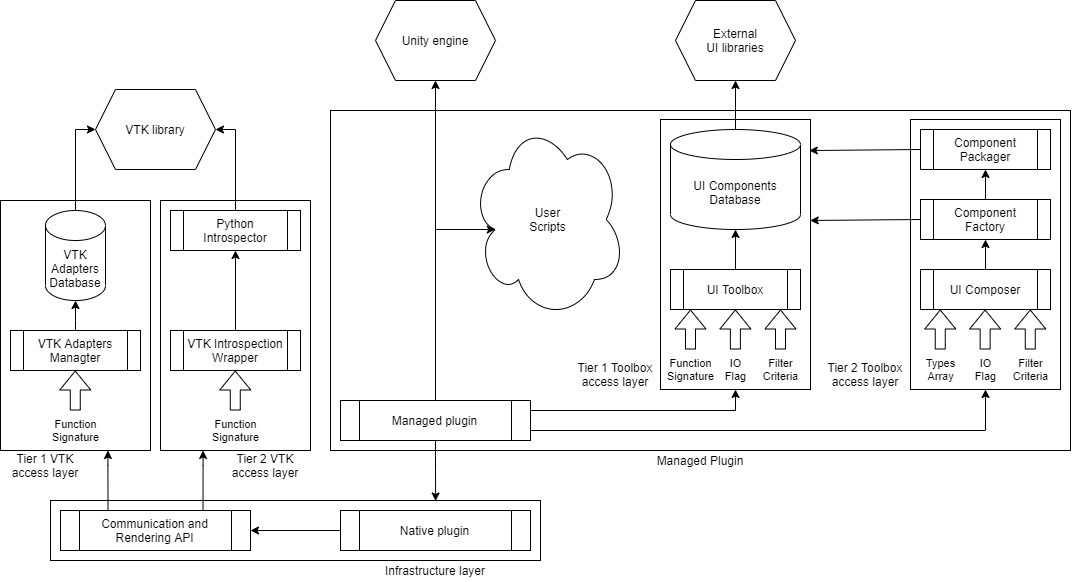
\includegraphics[width=\textwidth]{pictures/Architecture-v0.3.png}
    \caption{The architecture design of the plugin, showing inner working details of the various components.}
    \label{fig:high-level-architecture}
\end{figure}

\section{Infrastructure}
\label{sec:design-infrastructure}

The first component we tackle is the most simple yet the most crucial of this plugin. The infrastructure layer acts as a dispatcher for the requests coming from the managed plugin, routing them either to the rendering API or further down towards the VTK access components. As a reference, the component is highlighted in the architecture in Figure~\ref{fig:arch-infra}

\begin{figure}
    \centering
    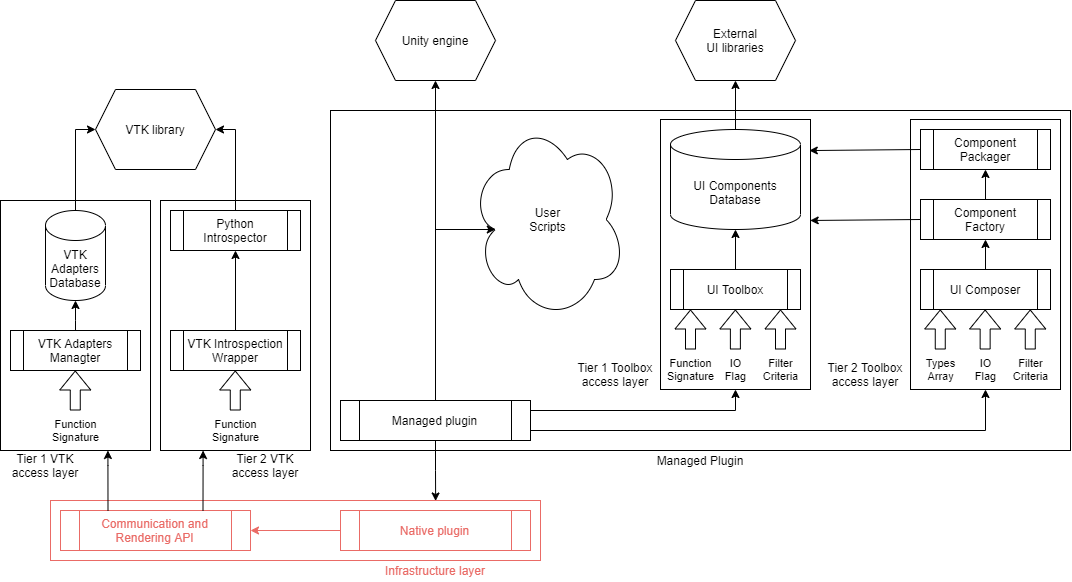
\includegraphics[width=\textwidth]{pictures/Architecture-v0.3-infra.png}
    \caption{Architecture with the infrastructure layer highlighted.}
    \label{fig:arch-infra}
\end{figure}

The infrastructure layer is the component responsible for allowing interaction between all other parts of the system. Its main job is to give a common entry-point to the \acrshort{vtk} interfaces and decide which to call, acting as a dispatcher. As this is the critical point of the system where communication flows, it is also the one that mostly affects parallelization and distribution capabilities. Thus, the calls should be as little blocking as possible, allowing flows to stop only at endpoints and not in the middleware.

Wheeler et al.'s VtkToUnity \cite{wheeler_virtual_2018} already partly implements this infrastructure layer and already exposes part of the \acrshort{vtk} interface as well. Unfortunately, their calls are highly blocking, as once the C++ native code executes, the Plugin calls each \verb|lock()| on the API and thus parallel calls are impossible. On the other hand, the plugin achieves decent performances that fall within the Unity guidelines for \acrshort{vr} \cite{unity_vr_2020}, while allowing for good maintainability and extension possibilities.

As such, we base the infrastructure layer on a refactoring of the VtkToUnity plugin which aims at the following results:

\begin{enumerate}
    \item Decoupling of the communication and dispatching from the interfacing responsibilities;
    \item Refactoring the interfacing code in adapters that constitute the foundation of the adapter-based interfacing;
    \item Move as much business logic of the infrastructure in non-blocking calls, preferably with no blocking at the infrastructure layer;
    \item Move blocking logic at interface level.
\end{enumerate}

%As we expect the interfacing to be slower, especially with the introspection component, the infrastructure layer will also have a cache system to store and retrieve the latest hits and directly call the precise function rather than going through with the introspecting dispatch system.

We use the same approach as in the VtkToUnity plugin to create the C++ native plugin and its interfacing with Unity. Our implementation is then reduced to the minimal API necessary to use the \acrshort{vtk} functionality expressed by the interface mechanisms described in Section~\ref{sec:design-interfaces}. Our objective is to make the calls as general as possible, giving the user the most liberty and access as possible. For the naming and implementation, we follow a similar design as the Python/C API \cite{python_c_api}. The interface is documented in Appendix~\ref{apx:api}.

In order to keep the readability and intuitiveness of the system decent, we apply this same approach to the API of all components. This is to limit the parsing operations, so that middleware has to apply as little transformation to the parameters as possible, as well as to make the maintainability of the system easier, as understanding data flows and meaning of values becomes easier with consistent naming and patterns.

\section{VTK Interfaces}
\label{sec:design-interfaces}

The core feature of our system is its ability to access \acrshort{vtk} and expose it fully to the \acrshort{vr} development environment. To achieve this, while keeping the system easily maintainable and performing, we use a two way access system. The first access route uses a lookup to check whether custom adapters exist that can satisfy the request from the caller, while the second uses introspection capabilities on the library to find the appropriate method, function or class that can satisfy the request.

We discuss both access tiers and how each of them is designed. Both these subsystems are intended to be separate services that the main architecture can either directly access when running in a stand-alone version on the users PC, or can be distributed on a network and be accessed through distribution engines such as DtCraft \cite{huang2017dtcraft} or Boost::MPI \cite{schaling2011boost}.

In order to limit the amount of routes in the infrastructure level and overheads, the interfaces follow a strict prioritization policy. The first tier is the Adaptrs registry, where a number of custom written adapters can be added and used by the plugin. If the infrastructure finds a suitable adapter, it will use it to answer the request. If no adapter is available, the query will be sent to the Introspection layer to be computed. However, if an adapter is found but it cannot satisfy the request, the system will not query the Introspection layer. Instead, it will return an error and it will be the user's responsibility to either query the Introspection layer directly or to expand the adapter. Other than the performance rationale behind this choice, the other main reason is that complexity in our system is kept at the peripheral components, with the clear intent of the dispatcher to be as simple and straight-forward as possible, limiting complexity in that central middleware.

\subsection{Introspection}
\label{sec:design-introspection}

The introspection layer is the low priority of the two VTK access tiers. It acts as the main route to connect to VTK and access its features and the most used component of the native part of our plugin for the average use-case of this system. It is comprised of two main parts, the Python \verb|Introspector| script, which uses the Dreuning implementation to access VTK introspectively, and the C++ wrapper that handles the memory used by the VTK objects and the Python Interpreter embedded in the system. As a reference, the component is highlighted in the architecture in Figure~\ref{fig:arch-intro}

\begin{figure}
    \centering
    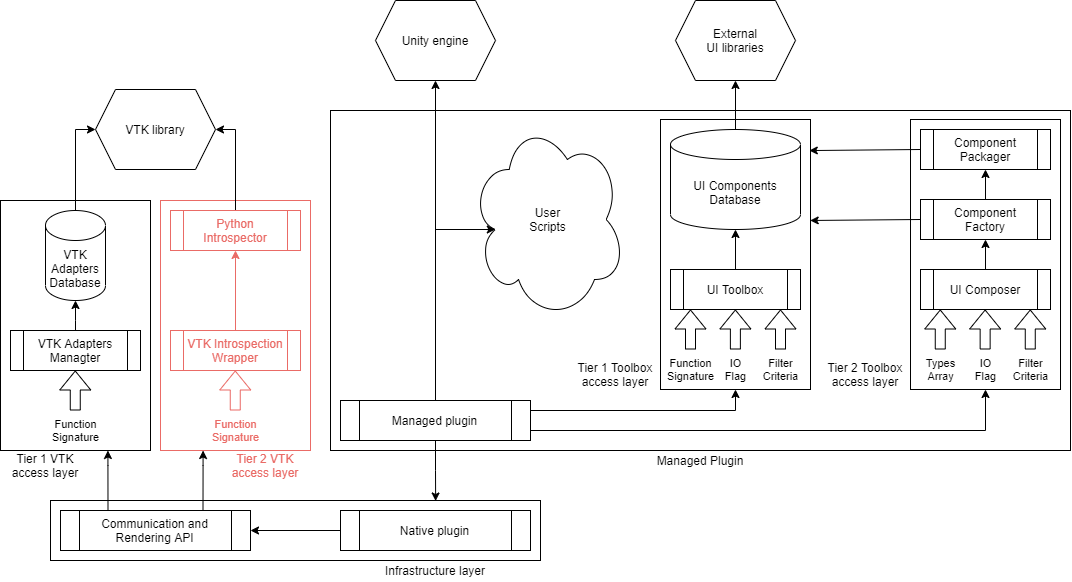
\includegraphics[width=\textwidth]{pictures/Architecture-v0.3-intro.png}
    \caption{Architecture with the introspection layer highlighted.}
    \label{fig:arch-intro}
\end{figure}

\subsubsection{Design}

As we discussed in Section~\ref{sec:rqrmsandclngs-challenges}, solutions already exist that implement introspective systems to access VTK in Python. In particular, we modify and extend the Python scripts from Dreuning's solution in order to make use of its \verb|ClassTree|. The issue we find with this implementation is that it is limited to \verb|vtkAlgorithm| classes, and as such leaves out a chunk of the features of the VTK. As extending these scripts is out of the scope of this thesis, we instead introduce a feature to overcome this limitation that would nevertheless be implemented, i.e. the ability to pipe the result of a VTK call to other calls. This does not allow the user to instantiate objects of classes that are not \verb|vtkAlgorithm|, however it allows already for a big part of the left out features to be accessed.

From Dreuning's solution we adapt the \verb|ClassTree| implementation in order to strip it of its UI related code, as well as the \verb|PipelineObject|, which we use as the introspective wrapper for the \acrshort{vtk} objects we instantiate to hold the getter and setter calls. A further script has been produced to facilitate the calls from C++, exposing the required features for: (a) creating a (wrapped) \acrshort{vtk} object and return the C++ object's address; (b) getting the description of a \acrshort{vtk} object, i.e. its attributes and their types, used by the Composer to generate UIs on-the-fly; (c) get the value of a \acrshort{vtk} object's attribute; (d) set the value of a \acrshort{vtk} object's attribute; and (e) delete the wrapper's information once the \acrshort{vtk} object gets deleted in the environment. 

In order to access the Python scripts from the C++ native plugin, we embed the Python 3.7 interpreter in the C++ implementation. This is achieved by initializing the interpreter as part of the process, using a subset of the software's memory to run Python. This, combined with the ability to wrap the C++ VTK objects using the \verb|vtkPythonUtils| class into Python and then access them back again, allows us not to worry about synchronizing memory and processes, boosting both memory and time performances.

The implementation instantiates a \verb|Introspector| class from Python, using it as access-point for the introspective methods. Using the \verb|PyObject_CallMethod| we are able to use the methods of the \verb|Introspector|, starting with \verb|createVtkObject| which instantiates a wrapped VTK object, using the class name, that carries the information of the getter and setter methods of the \verb|vtkAlgorithm| class. These wrapped objects, that we will now call \textit{nodes}, are registered in a structure that maps the pointer of the C++ object to its wrapped Python counterpart, for fast lookup access \cite{stdunord16}. The C++ interface exposes calls that allow, having the node available, to call getters, setters, to execute the VTK update of the object, retrieve the output port, delete the object, execute a generic or piped call. This last one means that you can execute, for example, \verb|object.GetOutput().GetCenter()| with a single access to the \verb|Introspector| and use non introspectable objects as intermediate values, expanding the possible calls that the plugin can execute.

To avoid ambiguity when calling these methods, and to avoid passing excessive data through the Unity native interface, the methods that retrieve values from the \verb|Introspector| use a postfix notation to determine whether the call is to return a native value that can easily be parsed to and from a string representation (\verb|_AsString|), an id of a VTK object (\verb|_AsVtkObject|), or either if the result is to be discarded or the method being called has \verb|void| return type (\verb|_AsVoid|).

When calling any method that uses parameters of generic types, we use a similar convention as the Python/C API so to make the maitainability of the code easier, as these are strictly intertwined and usually used alongside. As such, calls are structured as follows: the first parameter is the pointer to the object on which the method is to be called, the second parameter is the name of the method to be called, or a specifier that acts as a dispatching value (i.e. dispatching either to \verb|SetInputConnection| or \verb|SetSourceConnection|), third is the string format of the following parameters (e.g. a method that has three doubles as parameters would have as format \verb|"fff"|), and finally a vector containing the parameters. Special treatment is reserved for the \verb|"O"| object parameters that are first past as string representation of integer values, then parser to integers by the infrastructure layer, which represents the id of the VTK object in the registry, and finally two vectors are sent to the introspection layer, one with the \verb|vtkObjectBase *| objects and the other with the rest of the parameters.

A complete description of the formatting values see Table~\ref{tab:format-values}, while the interface of the introspection layer is documented in Appendix~\ref{apx:api}

\begin{table}[t]
    \centering
    \begin{tabulary}{.9\textwidth}{LL}
    \multicolumn{1}{c}{\textbf{Symbol}} & \multicolumn{1}{c}{\textbf{Meaning}} \\ \hline
    O & A VTK object. The value from the Managed plugin is the ID of the object in the infrstructure layer's registry. The Introspection layer receives the pointer to the VTK object. \\
    d                                   & A C integer or long value.           \\
    f                                   & A C float or double value.           \\
    s                                   & A C char or LPCSTR value.            \\
    b                                   & A C++ bool value.                    \\
    \%\# & is any of the previous symbols, \# is the number of values. It represents a tuple of values, e.g.: f3 corresponds to (fff) in the Python/C API.
    \end{tabulary}
    \caption{Format symbols used in the calls to the plugin.}
    \label{tab:format-values}
\end{table}

\subsubsection{Benefits and Limitations}

The obvious benefit of this implementation is that it allows us to broadly achieve VTK-completeness in our system. The Python component gives the plugin access to the \verb|vtkAlgorithm| classes, and through piped calls to VTK it is possible to implement virtually any visualization a native application could make. The Introspector can instantiate all the necessary VTK objects using the \verb|genericCall| at Python level and as such it could potentially make the system strictly VTK complete. However, this would come at a great cost in terms of computation time, as all the information available for the \verb|vtkAlgorithm| classes is not generated.

A more subtle benefit of the usage of Python is that it is an interpreted language, and the interpreter being embedded in the C++ code makes it easier to maintain and expand the Introspector capabilities. Changes to such parts of the introspection layer would not require the plugin to be re-built everytime, whereas any change to the C++ code requires the plugin to be built and deployed in the Unity environment again. Furthermore, Python being a high level language, the actual implementation becomes more readable and understandable, making the component easier to work on.

As already introduced in Section~\ref{sec:design-infrastructure} on the infrastructure layer, we use a common convention on functions' and parameters' names and meaning, very similar to the Python/C API. Keeping this standard is not only beneficial to the maintainability of the system, as the code is easier to read, but also to its performances as the passage from our C++ to the Python/C API calls and viceversa is straight-forward, requiring limited parsing.

The API proposed does not limit the users ability to use VTK. Indeed, the calls that are exposed make no assumption on what the objects are used for and how, and they create as little barriers as possible. The main issue is that the calls support only a limited amount of types as parameters, compared to the Python/C API. On the other hand, these are representative of most of the types used within VTK classes and as such we believe this to be a minor limitation and that it does not impair our solution.

Lastly, thanks to the fact that most of the implementation of the C++ introspection layer uses little classes from VTK and mostly classes that tend to be not modified a lot by the VTK developers, like the \verb|vtkObjectBase| class, which is the root of all classes in the library. As such, updating the component to newer versions of VTK requires only the recompilation of the plugin and having the correct version of the Python wrapper installed on the machine.

The main limitation of this implementation is that it is not strictly VTK complete. Any class that is not inheriting from \verb|vtkAlgorithm| is not introspected on. These classes could be made available through generic calls through Python, but this would potentially introduce overheads at runtime that are not acceptable in such a performance critical system. As such, we accept this limitation of the system as it makes for a good compromise between our requirements of VTK completeness and performance. And thanks to the fact this is all achieved through Python, the system could potentially be made strictly VTK complete without touching the C++ code and as such left for future work.

\subsection{Adapters}
\label{sec:design-adapters}

Next to the introspection layer, the adapter layer is comprised of a collection of adapters added by the user. These are a way of allowing users to expand the plugin, taking advantage of the pure C++ performance edge over the C++ and Python introspection layer. Furthermore, it allows the users to introcude "templates" in the plugin, i.e. creating adapters that reduce repetitive and verbose calls to a single call to the C++ plugin. As a reference, the component is highlighted in the architecture in Figure~\ref{fig:arch-adapt}

\begin{figure}
    \centering
    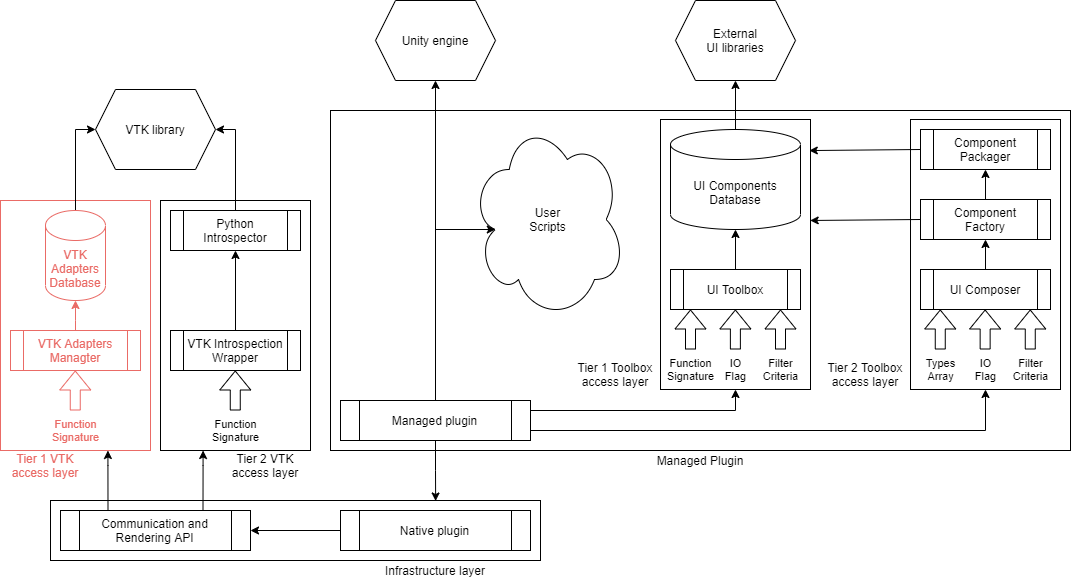
\includegraphics[width=\textwidth]{pictures/Architecture-v0.3-adapt.png}
    \caption{Architecture with the adapter layer highlighted.}
    \label{fig:arch-adapt}
\end{figure}

\subsubsection{Design}

The adapter layer is one of the two main ways in which expert users can tailor their experience with the system. These are pieces of C++ code that can be introduced in the native plugin's adapters folder and be called from the Unity environment. Particular use cases for adapters are:

\begin{enumerate}
    \item The creation of custom loggers for diagnostics and flow analysis;
    \item Implementation of \textit{templates} at native level that enable faster instantiation and define their own parameters and routines;
    \item Implementation of custom algorithms that compound \acrshort{vtk} features.
\end{enumerate}

The adapters are Singleton instances that define first and foremost a unique string identifying which component they are adapting. Such ID represents the name of the object the code adapts. For instance, an adapter for the  source class \verb|vtkConeSource| should be identified by the class' name. Furthermore, each adapter has to implement access methods for getting descriptions of what attributes the class has, getting the values of each of those attributes and setting such values as well. 

Optionally, the adapter can implement rendering information in case the adapter is not for a specific \acrshort{vtk} class but for a template or custom algorithm, in which case information is needed on how to render and update the objects generated by the adapter.

In order to implement the defined adapters, we first define a basic adapter class which is used for only use case number 1, i.e. the adapting of \acrshort{vtk} defined objects. This class does not define rendering and update information, as these are already defined by \acrshort{vtk}. We implement \verb|vtkAdapter| as shown in listing~\ref{lst:vtkadapter}

\begin{figure}[ht!]
    \centering
    \begin{cpp}[label=lst:vtkadapter,caption={vtkAdapter class}]
class vtkAdapter
{
public:
    template <typename T> using getter = std::stringstream(T::*)(vtkObjectBase *);
    template <typename T> using setter = void (T::*)(vtkObjectBase *, LPCSTR);

    virtual ~vtkAdapter() { }

    inline LPCSTR GetAdaptingObject() 
    {
        return m_vtkObjectName;
    }

    virtual void SetAttribute(
        vtkObjectBase *object,
        LPCSTR propertyName,
        LPCSTR newValue) = 0;

    virtual LPCSTR GetAttribute(
        vtkObjectBase *object,
        LPCSTR propertyName) = 0;

    virtual LPCSTR GetDescriptor() const = 0;

    virtual vtkObjectBase *NewInstance() = 0;

    virtual LPCSTR CallMethod_AsString(
        vtkObjectBase *object,
        LPCSTR method,
        LPCSTR format,
        const char *const *argv) const = 0;

    virtual vtkObjectBase *CallMethod_AsVtkObject(
        vtkObjectBase *object,
        LPCSTR method,
        LPCSTR format,
        const char *const *argv) const = 0;

    virtual void CallMethod_AsVoid(
        vtkObjectBase *object,
        LPCSTR method,
        LPCSTR format,
        const char *const *argv) = 0;

protected:
    // The name of the VTK object (as written in the wiki) for which
    // the class acts as an adapter
    LPCSTR m_vtkObjectName;

    vtkAdapter(
        LPCSTR vtkObjectName) 
    { 
        m_vtkObjectName = vtkObjectName;
    };
};
    \end{cpp}
\end{figure}

The class has a unique identifier in the form of a \verb|LPCSTR| (Long Pointer to Const STRing) which is to be set when instantiating the adapter. The class also carries with it a descriptor of the \acrshort{vtk} class that specifies what attributes the class has and what is their type. This descriptor is used by the Unity Managed plugin as we discuss in Section~\ref{sec:design-uicomposer}.

Alongside these functions, there are two templates that define the types of \verb|getter| and \verb|setter| methods used by adapters. These functions take as input a pointer to the actor that renders the \acrshort{vtk} object and the first returns a string representation of the value of the attribute while the second takes a further argument that is the new value to which attribute is to be set.

The generic calls for getting and setting attributes are respectively \verb|GetAttribute| and \verb|SetAttribute|. These functions act as dispatchers for the particular operations, that can either be directly implemented into the function but, as good practice, we later show an example of how we recommend these adapters should be implemented.

The actual attribute to change is encoded in a \verb|LPCSTR| that contains the name of the attribute exactly as written in the C++ code. A difference from the \verb|GetAttribute| generic call and the particular \verb|getter| template is that the return value is not returned but a specific parameter acts as return buffer, as this value is not to be used inside the C++ native code but to be sent through to the C\# interface in Unity.

Finally, the \verb|CallMethod| family of methods allows the user to implement generic methods that can be called from the Unity environment. In particular, these methods are meant to be used to accomodate the needs of use cases number 2 and 3. These use a similar signature to the \verb|VtkResource_CallMethod| methods from the plugin's API, so that the parameters can be directly passed down without the need of unnecessary parsing at the infrastructure level. The responsibility for correct parsing is left to the user to implement, so that they can also have a higher degree of freedom of what they can actually code.

Alongside the adapters, the \verb|vtkAdapterUtility| provides the access point for the register of the adapters. This allows to couple adapters to a single point of entry and masks the adapters to the infrastructure layer, making it easy to execute on a separate service. The implementation of this class is generated by a Python script at build time, available in Appendix~\ref{apx:generate-register}. The interface of the utility is shown in Listing~\ref{lst:vtkadapterutility}.

\begin{figure}[ht!]
    \centering
    \begin{cpp}[label=lst:vtkadapterutility,caption={vtkAdapterUtility interface}]
class vtkAdapterUtility
{
public:
	static vtkAdapter *GetAdapter(LPCSTR vtkAdaptedObject);

private:
	static const std::unordered_map<LPCSTR, vtkAdapter *> s_adapters;
};
    \end{cpp}
\end{figure}

As visible, the adapter only exposes the function \verb|GetAdapter| that returns the implementation of the adapter for the unique ID requested if such object exists, \verb|NULL| otherwise. The adapters are stored in an unordered map, as it has faster access times than the ordered counterparts \cite{stdunord16, stdmapcp55} on the average case. This depends on the hashing function, but as we use default types for keys and we do not replicate them, the average case is almost certainly guaranteed. The map is populated on instantiation and the entries are generated as Singletons, as shown in Listing~\ref{lst:adaptersmap}.

\begin{figure}[ht!]
    \centering
    \begin{cpp}[label=lst:adaptersmap,caption={Example of adapters register instantiation.}]
const std::unordered_map<LPCSTR, vtkAdapter*> vtkAdapterUtility::s_adapters =
{
	{ Singleton<vtkConeSourceAdapter>::Instance()->GetAdaptingObject(), Singleton<vtkConeSourceAdapter>::Instance() },
	// More adapters...
};
    \end{cpp}
\end{figure}

\subsubsection{Benefits and Limitations}

These adapters have the objective of allowing the user to customize their system and tailor it to their needs. The user can define different ways in which the native plugin interacts with \acrshort{vtk}. The ability to customize the software to this extents enables users to create code that can be re-used and distributed. Within a community of users, this allows them to exchange knowledge and tools that could not be achieved without this feature.

The main driver behind adapters is to make the solution maintainable as well as generic. We do not foresee all potential uses of the adapters, as it is not our objective. Their implementation is kept to the bare minimum and some use cases are presented which are, to us, the most obvious. We set out to not limit the potential for these components, and require the implementation of what is needed to make it work. This caters to our requirement of a usable system, as it makes it easier to tailor to specific needs of users.

The level of generality of this component however is also one of its main limitations. As we cannot foresee all the possible use-cases, and to avoid limiting users' options, we do not enforce many restrictions on what adapters can and cannot do. Furthermore, we can do little to enforce standards and recommended ways of using adapters, for the same reasons as before. As such, where users have great potential for new features, thay also have little support from the system to maintain and debug them.

Another limitation, at least compared to the introspection layer, is that this tier has no guarantee to compile with different versions of VTK, as the features used are not guaranteed to be present or be the same across versions. Although VTK developers have as one of their requirements the new versions of the library to be backwards compatible as already discussed in Chapter~\ref{ch:rqrmsandclngs}, this does not mean that they are forwards compatible, and adapters developed with newer versions of VTK are not guaranteed to work with older ones, and we do not set a way to solve this issue. This is because adapters are tools for the users and they should be responsible for paying attention to these kind of details.

The other great advantage of adapters over introspection is that it can make use of the performances of pure C++ code. As we discussed in Chapter~\ref{ch:rqrmsandclngs}, pure C++ code runnig VTK algorithms achieves far greater performances on the execution of pipelines than our approach using Python. As such, adapters enable the users to take advantage of such performances, removing the barrier of also having to code their Unity plugin along.

\section{Managed Plugin}
\label{sec:design-managed-plugin}

The integration of VTK with Unity makes use of both a native plugin, which we already discussed, and a managed plugin, which is the focus of this section. In particular, this part of the system is responsibile for making the native plugin API more user-friendly, and connecting the rendering cycles of the two rendering contexts. The setup is almost identical to the VtkToUnity plugin, with a different API for VTK.

The basic API of the managed plugin is identical to the native plugin API, with the exception of the usage of the \verb|Marshal|, a .NET library used to work with unmanaged memory areas. In Unity, this library is used in particular to handle passing paramters back and forth between the managed and native parts of the environment, like defining how strings have to be handled passing down to C++. In our implementation we use this exclusively to specify strings to be handled as long pointer strings, as we represent them as \verb|LPCSTR| (Long-Pointer Constant STRing) in our C++ code.

As a further design discussion, we present now the Toolbox and Composer components that are part of the managed plugin. As the UI is out of the scope of this thesis, we will not discuss particular implementations of these components, as they will be presented in a separate thesis. Designing these components, we mirror our approach to accessing VTK, as our drivers remain the same. In particular, the Toolbox is the component that mirrors the Adapters registry, while the Composer mirrors the Introspector.

For the API of the managed plugin, see Appendix~\ref{apx:api}. The minimal API is identical to the native plugin API, with the types being those of C\#, while the support and quality of life methods introduced in C\# to avoid verbose code is separately documented.

\subsection{UI Toolbox}
\label{sec:design-toolbox}

The UI Toolbox is the main access to UI components of the managed plugin. It acts as a database of factories that generate specific UIs when called upon. As a reference, the component is highlighted in the architecture in Figure~\ref{fig:arch-toolbox}

\begin{figure}
    \centering
    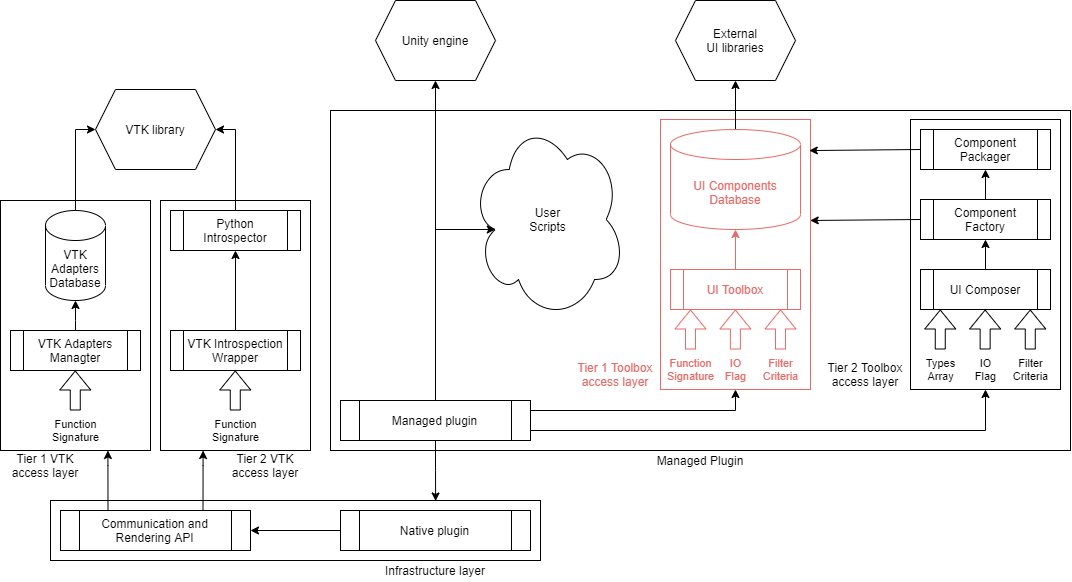
\includegraphics[width=\textwidth]{pictures/Architecture-v0.3-toolbox.png}
    \caption{Architecture with the UI Toolbox highlighted.}
    \label{fig:arch-toolbox}
\end{figure}

As UIs are in general more complex than accessing introspectively a library, as they are made of more components and constrained by interaction and usage limits that depend on the device being used, the environment, the input devices and so on, the ability to introduce custom-tailored UI components is necessary. Thus, we propose the usage of a registry of UI prefabs developed in Unity as first-tier access to the UI of the environment.

A registry mapping from the classname to the prefab factory \verb|IComponentFactory| acts as the access-point for the UI instantiation. When a part of the pipeline is created, the \verb|FactoryManager| first checks the registry to check whether a factory for the entire UI exists. If this exists, the factory is called and a \verb|Create| function generates the UI based on the prefab. The UI is then linked to the particular part of the pipeline by the manager in order to keep track of the changes and to avoid the changes being either lost or set to the wrong VTK object. This is also to have the UI ready but not shown, and only made visible through \verb|Show| when necessary and hidden through \verb|Hide| when changing focus.

\subsection{UI Composer}
\label{sec:design-uicomposer}

Finally, the UI Composer is the last part of the plugin we will discuss. This is a factory of factories, generating UI components that are a collection of minimal input UIs that are the base of the UI Toolbox. As a reference, the component is highlighted in the architecture in Figure~\ref{fig:arch-comp}

\begin{figure}
    \centering
    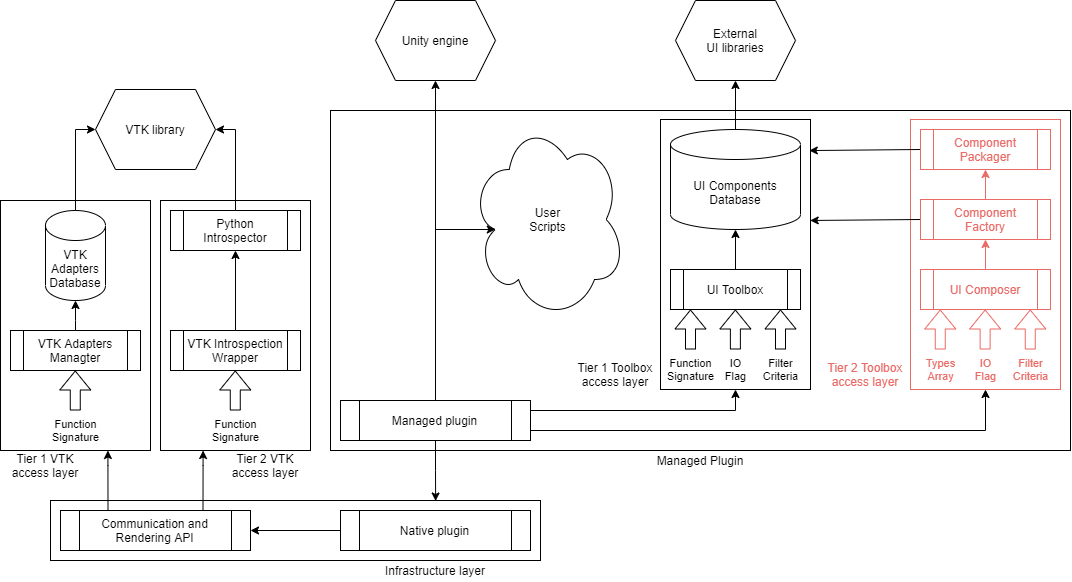
\includegraphics[width=\textwidth]{pictures/Architecture-v0.3-comp.png}
    \caption{Architecture with the UI Composer highlighted.}
    \label{fig:arch-comp}
\end{figure}

If the Toolbox fails, a generic system to generate UIs gets called. This requires more resources and time to execute, as it takes the descriptor of the VTK object, which maps the names of the attributes to their types, and then creates a minimal UI with this information. The Composer uses a registry of minimal components that are part of the environment that implement interfaces to edit native simple values, e.g. integers, decimals, booleans, strings and so on. These components are also registered with the Toolbox, for faster access.

The components generated this way are then used to instantiate a \verb|ComposedUI| object, that contains the information of the different parts that make the UI and then add this to the Composer's registry, acting as a \verb|IComponentFactory| for later calls of the \verb|FactoryManager| on the same classname to avoid generating the same factory twice.

In order to accelerate and expand the Composer's ability, the mappings are not hardcoded; the Composer still uses the Toolbox as a lookup for the basic parts used to generate the UI, and thus custom-tailored basic UIs can be added to the Toolbox to override the natively implemented ones. In this way, the component for a given string in the \verb|FactoryManager|'s registry is always the last one registered, making the native ones the lowest priority ones.

The \verb|FactoryManager| is designed in order to accomodate our maintainability driver, and as such this modular registry comes in handy to set some conventions in the development of UIs using this system that make them re-usable. In particular, UI components should be registered either if they allow the manipulation and/or visualization of a single parameter or when they combine other UI components. The first ones constitute the minimal set of the UI components, which respond to a particular input/output, like \verb|float|, \verb|int|, or \verb|string|, while the others respond to complex interactions like showing the UI for a \verb|vtkConeSource| object, or visualizing a \verb|stringList|. For the naming of the components we encourage camel case with the first letter lowercase as by VTK's convention. 

This conventions also make for the best operability of the Composer that will be able to generate more complex UIs, using composed UIs instead of simple input methods. To allow for further customization, we propose that the names can be postponed with filters that specify how the input is inserted, i.e. a float can be inputted through \verb|slider| or \verb|textField| for example. However, this is to make the modularity more useful to the user, rather than to the composer, as we do not design how these filters could be used by it.
